\chapter{Resultados}
\label{ch:resultados}

%* Comprobar
En el siguiente capitulo se van a comentar los diversos resultados obtenidos en el presente TFG, tanto los relacionados con la FPGA (\emph{hardware} usado, simulaciones y sintetizado final), como con el \emph{software} de control. Se incluyen además, varias imágenes que complementen las explicaciones del mismo.


%!
\section{Resultados de los elementos \emph{hardware} del sistema.}
%* Comprobar
Partiendo del esquema dado de analizadores USB \emph{hardware} (figura~\ref{fig:esquema-hardware}), se aprecian dos partes implicadas en la captura, por un lado el encargado de capturar la trama, y por otro, el encargado de controlar dicha captura y almacenar los resultados. En esta sección se van a comentar los resultados de la primera.

\begin{figure}[htb]
    \centering
    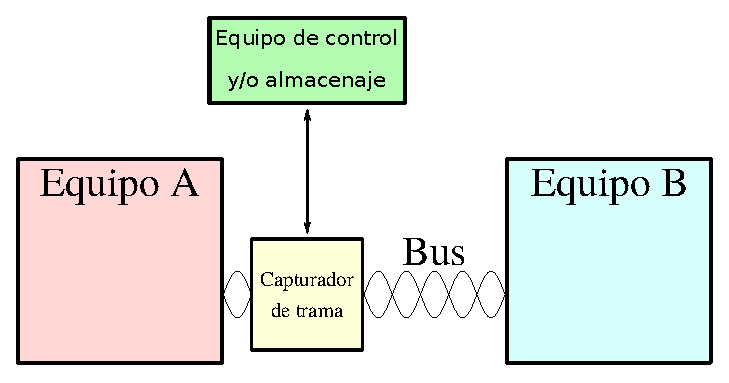
\includegraphics[width=70mm]{esquemas/esquema-captura-hardware-2.eps}
    \caption{Esquema de analizadores \emph{hardware}}
    \label{fig:esquema-hardware}
\end{figure}

%* Comprobar
\subsection{Componentes utilizados.}
En al figura \ref{fig:sistema_final} se muestra el resultado \emph{hardware} del presente trabajo, este a su vez, está formado por los siguientes componentes.

\begin{figure}[htbp]
    \centering
    \includegraphics[height=110mm]{hw_final/final_cut.jpg}
    \caption{Sistema de captura final}
    \label{fig:sistema_final}
\end{figure}

\begin{enumerate}
    %* Comprobar
    \item \textbf{Placa de desarrollo \emph{IceStick \cite{icestickmanual}} (Véase figura~\ref{fig:IceStick_board}).} \\
    Se trata de una placa de desarrollo, que incorpora, sin contar con todos los conectores, indicadores \emph{LEDs}, elementos pasivos y componentes de regulación, la \emph{FPGA iCE40HX-1k \cite{lattice:ice40}} del fabricante \emph{Lattice}\footnote{Página web del producto: \url{https://www.latticesemi.com/Products/FPGAandCPLD/iCE40.aspx}}, memoria SPI de $32MBit$ para almacenar el sintetizado generado, conversor USB a doble puerto de comunicación FIFO \emph{FTDI 2232H \cite{FTDI:FT2232HL}} para comunicarse con el PC y oscilador de $12MHz$ con el que referenciar ciertas partes del circuito.
    
    \begin{figure}[htbp]
        \centering
        \includegraphics[width=125mm]{hw_final/IceStick_board_cut.jpg}
        \caption{Placa de desarrollo \emph{IceStick}}
        \label{fig:IceStick_board}
    \end{figure}

    %* Comprobar
    \item \textbf{Módulo encargado de la capa física USB.} \\
    PCB que incorpora el circuito integrado \emph{USB3300\cite{icestickmanual}} del fabricante \emph{Microchip}. Este se encarga de manejar la capa física del bus USB, comunicándose con la FPGA por medio del protocolo ULPI\cite{ulpi-specs}.

    En al figura~\ref{fig:USB3300_board}, se aprecia que dicha PCB incluye dos conectores USB, uno tipo A hembra, y otro tipo mini-B hembra. Sus señales de datos están interconectadas, por lo que es en este punto donde ambos extremos del bus a analizar se unen, pudiendo capturar la trama sin interrumpir la conexión debido a que, el integrado \emph{USB3300} se puede configurar para mantener sus patillas de datos en alta impedancia.

    \begin{figure}[htbp]
        \centering
        \includegraphics[width=50mm]{hw_final/USB3300_board_cut.jpg}
        \caption{PCB con el integrado \emph{USB3300}}
        \label{fig:USB3300_board}
    \end{figure}

    %* Comprobar
    \item \textbf{Cableado de unión (Figura~\ref{fig:matriz-hw-resto:cables}).} \\
    Para conexionar ambas placas, se utilizan varios cables entre el conector del módulo con el integrado \emph{USB3300} y los conectores laterales de la placa \emph{IceStick}.

    La \emph{FPGA iCE40HX-1k} posee 4 bancos de señales de entrada/salida, para evitar posibles retrasos en las señales\cite{fpga:routing}, los 8bits de datos paralelos se conectan al banco 0 (pines del 112 al 119), mientras que el resto de señales ULPI (DIR, STP, RST y NXT) al banco 2.
    
    %* Comprobar
    \item \textbf{Pulsadores externos (Figura~\ref{fig:matriz-hw-resto:botones}).} \\
    Se han incluido dos botones auxiliares externos, con los que poder tanto reiniciar el sistema en su totalidad, como enviar un $byte$ de prueba por el puerto serie.
    
    Las señales son activas a nivel bajo, por lo que se mantienen siempre a nivel alto por medio de unas resistencias de \emph{Pull-Up} (Figura~\ref{fig:buttons_circuit}).
    \begin{figure}[h]
        \centering
        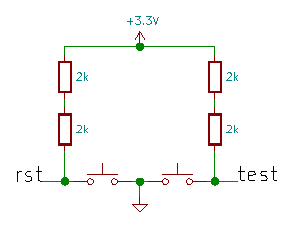
\includegraphics[width=50mm]{hw_final/buttons_circuit2.eps}
        \caption{Esquema de los botones auxiliares}
        \label{fig:buttons_circuit}
    \end{figure}

    %* Comprobar
    \item \textbf{Base impresa en 3D (Figura~\ref{fig:matriz-hw-resto:base}).} \\
    Para facilitar el trabajo, se ha diseñado con SolveSpace\footnote{Herramienta de diseño parámetro CAD 2D/3D. \url{http://solvespace.com}}, y posteriormente impreso, una pequeña base en 3D, en la cual tener las dos placas unidas y organizadas.

    \begin{figure}[!htb]
        \centering
        \subfigure[Cables de interconexión]{
            \includegraphics[height=40mm]{hw_final/cables_cut.jpg}
            \label{fig:matriz-hw-resto:cables}
        }
        \subfigure[Botones auxiliares]{
            \includegraphics[height=40mm]{hw_final/buttons_cut.jpg}
            \label{fig:matriz-hw-resto:botones}
        } \\
        \subfigure[Base 3D]{
            \includegraphics[height=75mm]{hw_final/3D_base.jpg}
            \label{fig:matriz-hw-resto:base}
        }
        \caption{Resto de elementos usados en el sistema de captación} 
        \label{fig:matriz-hw-resto}
    \end{figure}
\end{enumerate}

%!
\subsection{Módulos integrados en la FPGA.}
Siguiendo los objetivos planteados en el capitulo~\ref{ch:objetivos}, se han diseñado e implementado los siguientes módulos en la FPGA, todos en lenguaje Verilog.

\textbf{Nota.} En el anexo~\ref{ch:diagramas} se muestran de forma gráfica todas las relaciones existente entre ellos, mientras que en el anexo~\ref{ch:maquinas-estados} se plasman sus maquinas de estados \emph{Mealy} internas.

%* Comprobar
\subsubsection{Módulo divisor de reloj (clk\_div).}
Módulo que divide un reloj de entrada, tal que la frecuencia de salida sea $f_{out} = \frac{f_{in}}{2^n}$, donde $n$ es el número de \emph{Flip-Flops} tipo D utilizados, como se aprecia en la figura~\ref{fig:clk_div_esquema}. En el listado~\ref{src:resultados-modulos-clk-div} se plasman los parámetros, entradas y salidas del módulo.

\begin{figure}[hbt]
    \centering
    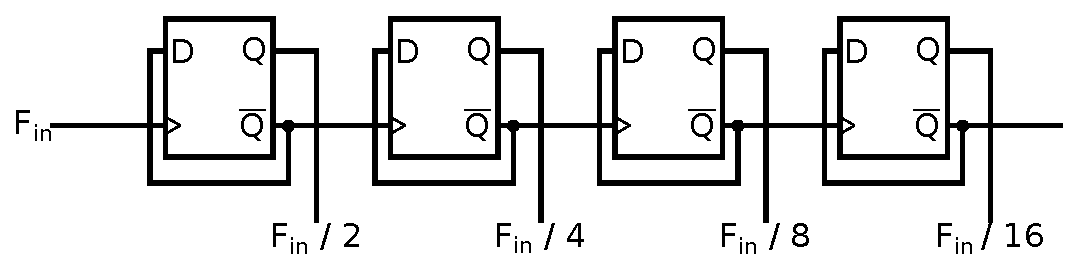
\includegraphics[width = 90mm]{esquemas/divisor_flipflop_D.eps}
    \caption{Divisor de reloj con \emph{Flip-Flops}}
    \label{fig:clk_div_esquema}
\end{figure}

A partir de él se generan dos relojes, uno basado en el reloj de $12MHz$ procedente de la placa \emph{iCEstick} (señal llamada clk\_div\_ice) y otro a partir del reloj de $60MHz$ del módulo USB3300 (señal  llamada clk\_div\_ULPI). Ambos relojes se dividen 24 veces y su única funcionalidad es la de  comprobar el funcionamiento del sistema por medio de los LEDs integrados en la placa.

\begin{lstlisting}[language=Verilog,
    caption={Parámetros, entradas y salidas del módulo clk\_div.},
    label=src:resultados-modulos-clk-div]
/*
 *
 * Módulo clk_div
 *
 * Parámetros:
 *  - DIVIDER. Número de veces que el reloj de referencia es dividido. f_clk_out = f_clk_in / (2^DIVIDER)
 *
 * Entradas:
 *  - enable. Cuando esta señal esté a nivel alto, el módulo estará activo, y en caso contrario la salida estará siempre a nivel bajo.
 *  - clk_in. Reloj de referencia a partir del cual se genera el de salida.
 *
 * Salidas:
 *  - clk_out. Señal de reloj generada con la frecuencia deseada.
 *  - clk_pulse. Señal con la misma frecuencia que el reloj de salida, pero con un ancho de pulso igual al del reloj de entrada.
 *
 */
\end{lstlisting}

% Parámetros:
% \begin{itemize}
%     \item \textbf{DIVIDER.} Número de veces que el reloj de referencia es dividido.
% \end{itemize}

% Entradas:
% \begin{itemize}
%     \item \textbf{enable.} Cuando esta señal esté a nivel alto, el módulo estará activo, en caso contrario, la salida estará siempre a valor bajo.
%     \item \textbf{clk\_in.} Reloj de referencia a partir del cual se genera el de salida.
% \end{itemize}

% Salidas:
% \begin{itemize}
%     \item \textbf{clk\_out.} Señal de reloj generada con la frecuencia deseada.
%     \item \textbf{clk\_pulse.} Señal con la misma frecuencia que el reloj de salida, pero con un ancho de pulso igual al del reloj de entrada.
% \end{itemize}


%* Comprobar
\subsubsection{Módulo de generación de reloj de baudios (clk\_baud\_pulse).}
De igual manera que el módulo divisor de reloj, este también genera uno, pero en esta ocasión en vez de utilizar directamente \emph{Flip-Flops}, se utiliza un contador, lo que permite una mayor precisión en la salida, con un ancho de pulso igual al del reloj de entrada. En el listado~\ref{src:resultados-modulos-clk-baud-pulse} se plasman los parámetros, entradas y salidas del módulo.

Este reloj generado, configurable por medio de un parámetro de entrada, es usado para controlar la velocidad (baudios) de lectura/escrituro en el módulo de comunicación serie, comentado más adelante.

\begin{lstlisting}[language=Verilog,
    caption={Parámetros, entradas y salidas del módulo clk\_baud\_pulse.},
    label=src:resultados-modulos-clk-baud-pulse]
/*
 *
 * Módulo clk_baud_pulse
 *
 * Parámetros:
 *  - COUNTER_VAL. Valor optimo a contar para generar el pulso deseado.
 *  - PULSE_DELAY. Numero de retrasos en la señal de salida antes producir un pulso.
 *
 * Entradas:
 *  - enable. Cuando esta señal esté a nivel alto, el módulo estará activo, y en caso contrario la salida estará siempre a nivel bajo, reiniciando además sus registros internos.
 *  - clk_in. Reloj de referencia a partir del cual se genera el de salida.
 *
 * Salidas:
 *  - clk_pulse. Pulso generado.
 *
 */
\end{lstlisting}


%* Comprobar
\subsubsection{Módulo de memoria FIFO (FIFO\_BRAM\_SYNC).}
Módulo que de forma sincrona en lectura y escritura al reloj, es capaz de almacenar datos en los bloques de RAM internos de la FPGA, de tal manera que el primer dato en ser introducido sea el primero en ser extraído. En el listado~\ref{src:resultados-modulos-fifo} se plasman los parámetros, entradas y salidas del módulo.

Se han creado dos variantes, FIFO\_BRAM\_SYNC y FIFO\_BRAM\_SYNC\_CUSTOM, ambas parten de la misma base de funcionamiento, pero la segunda permite utilizar más de un único bloque de RAM interna.

\begin{lstlisting}[language=Verilog,
    caption={Parámetros, entradas y salidas del módulo FIFO\_BRAM\_SYNC\_CUSTOM.},
    label=src:resultados-modulos-fifo]
/*
 *
 * Módulo FIFO_BRAM_SYNC_CUSTOM
 *
 * Parámetros:
 *  - ALMOST_FULL. Porcentaje mínimo de la memoria que hace que se active la señal wr_almost_full. Por defecto vale 0.9.
 *  - ALMOST_EMPTY. Porcentaje máximo de la memoria que hace que se active la señal rd_almost_empty. Por defecto vale 0.1.
 *  - DATA_WIDTH. Tamaño de cada valor almacenado. Por defecto vale 8bits.
 *  - FIFO_SIZE_ML. Número de bloques de RAM a usar. Por defecto se utiliza uno.
 *
 * Entradas:
 *  - rst. Señal de reinicio, activa a nivel bajo.
 *  - clk. Reloj de referencia.
 *  - wr_dv. Señal que indica que los datos de entrada deben ser almacenados.
 *  - wr_DATA. Datos a ser almacenados. Debe tener el mismo ancho que el parámetro DATA_WIDTH.
 *  - rd_en. Señal que indica que se desea leer los datos almacenados.
 *
 * Salidas:
 *  - wr_full. Señal que indica que la memoria esta llena. Futuras operaciones de escritura serán ignoradas.
 *  - wr_almost_full. Señal que indica que la memoria esta casi llena.
 *  - rd_DATA. Datos leidos de la memoria.
 *  - rd_empty. Señal que indica que la memoria esta vacía. Futuras operaciones de lectura serán ignoradas.
 *  - rd_almost_empty. Señal que indica que la memoria esta casi vacía.
 *
 */
\end{lstlisting}

% Parámetros:
% \begin{itemize}
    %     \item \textbf{\emph{ALMOST\_FULL}.} Porcentaje mínimo de la memoria que hace que se active la señal wr\_almost\_full. Por defecto vale $0.9$.
    %     \item \textbf{\emph{ALMOST\_EMPTY}.} Porcentaje máximo de la memoria que hace que se active la señal rd\_almost\_empty. Por defecto vale $0.1$.
    %     \item \textbf{\emph{DATA\_WIDTH}.} Tamaño de cada valor almacenado. Por defecto vale $8~bits$.
% \end{itemize}
% Entradas. Señales sincrona al flanco de subida del reloj.:
% \begin{itemize}
    %     \item \textbf{\emph{rst}.} Señal de reinicio, activa a nivel bajo.
%     \item \textbf{\emph{clk}.} Reloj de referencia.
%     \item \textbf{\emph{wr\_dv}.} Señal que indica que los datos de entrada deben ser almacenados. 
%     \item \textbf{\emph{wr\_DATA}.} Datos a ser almacenados. Debe tener el mismo ancho que el parámetro \emph{DATA\_WIDTH}.
%     \item \textbf{\emph{rd\_en}.} Señal que indica que se desea leer los datos almacenados.
% \end{itemize}
% Salidas:
% \begin{itemize}
%     \item \textbf{\emph{wr\_full}.} Señal que indica que la memoria esta llena. Futuras operaciones de escritura serán ignoradas.
%     \item \textbf{\emph{wr\_almost\_full}.} Señal que indica que la memoria esta casi llena.
%     \item \textbf{\emph{rd\_DATA}.} Datos leidos de la memoria.
%     \item \textbf{\emph{rd\_empty}.} Señal que indica que la memoria esta vacía. Futuras operaciones de lectura serán ignoradas.
%     \item \textbf{\emph{rd\_almost\_empty}.} Señal que indica que la memoria esta casi vacia.
% \end{itemize}


%* Comprobar
\subsubsection{Módulo de registro de desplazamiento universal (shift\_register).}
Submódulo capaz de desplazar tanto a izquierda como a derecha la información almacenada, y que a su vez, permita una carga y lectura en paralelo. En el listado~\ref{src:resultados-modulos-shift} se plasman los parámetros, entradas y salidas del módulo.

La finalidad de este submódulo es poder convertir datos de serie a paralelo o de paralelo a serie, cuando ocurra una recepción o transmisión respectivamente.

En la figura~\ref{fig:shift_esquema} se muestra, mostrando sus señales, el funcionamiento del registro de desplazamiento diseñado, en está ocasión, con desplazamiento hacia la derecha.

\begin{figure}[htb]
    \centering
    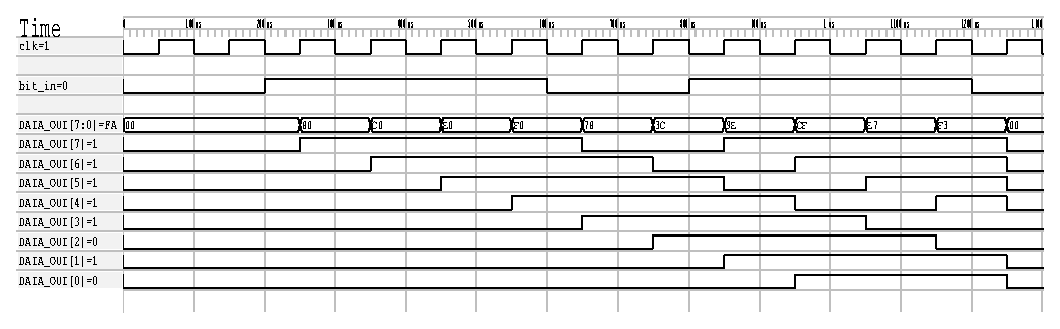
\includegraphics[height=46mm]{esquemas/shift_register.eps}
    \caption{Ejemplo de funcionamiento del registro de desplazamiento hacia la derecha.}
    \label{fig:shift_esquema}
\end{figure}

\begin{lstlisting}[language=Verilog,
    caption={Parámetros, entradas y salidas del módulo shift\_register.},
    label=src:resultados-modulos-shift]
/*
 *
 * Módulo shift_register
 *
 * Parámetros:
 *  - BITS. Tamaño en bits del registro de desplazamiento. El tamaño total será de BITS + 1 (bit de salida).
 *
 * Entradas:
 *  - clk. Reloj de referencia. Todas las operaciones se ejecutarán en el flanqueo de subida.
 *  - rst. Señal de reinicio, activa a nivel bajo.
 *  - bit_in. Bit a ser desplazado dentro del registro (modos 01 y 10).
 *  - DATA_IN. Datos a ser cargados de forma paralela (modo 11).
 *  - mode. Selector de operación a realizar [2 bits].
 *     > 00. No hacer nada.
 *     > 01. Desplazamiento a izquierda.
 *     > 10. Desplazamiento a derecha.
 *     > 11. Carga paralela.
 *
 * Salidas:
 *  - bit_out. Bit de salida tras el desplazamiento (modos 01 y 10).
 *  - DATA. Datos paralelos almacenados.
 *
 */
\end{lstlisting}


%* Comprobar
\subsubsection{Módulo de comunicación serie (UART).}
Sistema capaz de generar y recibir señales compatibles con una comunicación bidireccional serie 8N1\footnote{8N1: $8~bits$ de datos, sin $bit$ de paridad y un $bit$ de parada}, consiguiendo una tasa de transferencia estable máxima de $3750000~bauds$. Además, tanto para la lectura coma para la escritura, se han incorporado unos \emph{buffers} basados en memorias FIFO de $512~bytes$ cada uno. En el listado~\ref{src:resultados-modulos-uart} se plasman los parámetros, entradas y salidas del módulo.

Este módulo se ha dividido a su vez en los siguientes submódulos.
\begin{itemize}
    %* Comprobar
    \item \textbf{Submódulo de recepción serie (UART\_Rx).} \\
    Está continuamente esperando a que la señal de entrada de datos serie pase de un nivel alto a otro bajo, y una vez detectada esa caída, empezar a almacenar los $bits$ que conforman la trama a la velocidad dictada por el reloj de baudios. En la figura~\ref{fig:flujo_uart_rx} se muestra su flujo de funcionamiento.

    \begin{figure}[!hbt]
        \centering
        \scalebox{0.85} {\begin{tikzpicture}[auto]
    % Config
    \tikzFlow

    % Place nodes
    \node [flowStart] (idle) {Reposo};
    
    \node [flowDecision] at ($ (idle)+(0,-2.65) $) (rxLow) {Entrada del puerto serie a nivel bajo?};
    
    \node [flowBase, below of=rxLow] (init) {Reinicio del contador de $bits$};
    
    \node [flowBase] at ($ (rxLow.east)+(3.85,1) $) (read) {Se guarda $bit$ entrante en el registro de desplazamiento};

    \node [flowDecision, below of=read] (10bitsDone) {Se han leído los $10~bits$ del mensaje?};
    
    \node [flowBase] at ($ (read)+(4.1,0) $) (increase) {Incremento del contador de $bits$};

    \node [flowBase] at ($ (10bitsDone)+(4.1,0) $) (wait) {Se espera un pulso del reloj de baudios};

    \node [flowBase, below of=10bitsDone] (save) {Se almacena el byte en memoria};

    % % Draw edges
    \path [flowLine] (idle) -- (rxLow);
    \path [flowLine] (rxLow) -- (init);
    \path [flowLine] (init.south) |- +(3.5,-1) |- (read.west);
    \path [flowLine] (read) -- (10bitsDone);
    \path [flowLine] (increase) -- (read);
    
    \node [flowHide] at ($ (idle)+(2.75,0) $) (anchor1) {};
    \path [flowLine] (rxLow) -- node [right, xshift=-1.2cm] {Sí} (init);
    \path [flowLine] (rxLow.east) node [above, xshift=0.2cm] {No} -| (anchor1.center);
    
    \path [flowLine] (save.east) -| +(4.5,0) |- (idle.east);
    
    \path [flowLine] (wait) -- (increase);
    \path [flowLine] (10bitsDone.east) node [above, xshift=0.2cm] {No} -- (wait);
    \path [flowLine] (10bitsDone) -- node [right, xshift=-1.2cm] {Sí} (save);
\end{tikzpicture}


% \begin{tikzpicture}[auto]
%     % Config
%     \tikzFlow

%     % Place nodes
%     \node [flowStart] (idle) {Reposo};
    
%     \node [flowDecision, below of=idle] (rxLow) {Entrada del puerto serie a nivel bajo?};
    
%     \node [flowBase, below of=rxLow] (init) {Reinicio del contador de $bits$};
    
%     \node [flowBase, below of=init] (read) {Se guarda $bit$ entrante en el registro de desplazamiento};

%     \node [flowDecision, below of=read] (10bitsDone) {Se han leído los $10~bits$ del mensaje?};
    
%     \node [flowBase] at ($ (read)+(4.1,0) $) (increase) {Incremento del contador de $bits$};

%     \node [flowBase] at ($ (10bitsDone)+(4.1,0) $) (wait) {Se espera un pulso del reloj de baudios};

%     \node [flowBase, below of=10bitsDone] (save) {Se almacena el byte en memoria};

%     % % Draw edges
%     \path [flowLine] (idle) -- (rxLow);
%     \path [flowLine] (rxLow) -- (init);
%     \path [flowLine] (init) -- (read);
%     \path [flowLine] (read) -- (10bitsDone);
%     \path [flowLine] (increase) -- (read);
    
%     \node [flowHide] at ($ (idle)+(3.5,0) $) (anchor1) {};
%     \path [flowLine] (rxLow) -- node [right, xshift=-1.2cm] {Sí} (init);
%     \path [flowLine] (rxLow.east) -| node [above, xshift=-1.2cm] {No} (anchor1.center);
    
%     \path [flowLine] (save.east) -| +(4.5,0) |- (idle.east);
    
%     \path [flowLine] (wait) -- (increase);
%     \path [flowLine] (10bitsDone.east) node [above, xshift=0.2cm] {No} -- (wait);
%     \path [flowLine] (10bitsDone) -- node [right, xshift=-1.2cm] {Sí} (save);
% \end{tikzpicture}}
        \caption{Diagrama de funcionamiento del submódulo de recepción serie}
        \label{fig:flujo_uart_rx}
    \end{figure}
    
    %* Comprobar
    \item \textbf{Submódulo de emisión serie (UART\_Tx).} \\
    En este caso, cuando internamente se quiera enviar un mensaje, se exportan sucesivamente los $10bits$ que conforman la trama a la velocidad dada por el reloj de baudios. En la figura~\ref{fig:flujo_uart_tx} se muestra su flujo de funcionamiento.
    \begin{figure}[!hbt]
        \centering
        \scalebox{0.85} {\begin{tikzpicture}[auto]
    % Config
    \tikzFlow

    % Place nodes
    \node [flowStart] (idle) {Reposo};
    
    \node [flowDecision, below of=idle] (newData) {Existen datos a enviar?};

    \node [flowBase, below of=newData] (reset) {Reinicio del contador de $bits$};
    
    \node [flowStart, below of=reset] (load) {Carga de datos a enviar en el registro de desplazamiento};
    
    \node [flowStart, below of=load] (sendBit) {Se envía un bit, y se desplaza el registro};
    
    \node [flowDecision, below of=sendBit] (done) {Se han enviado los 10 bits del mensaje?};
    
    \node [flowBase] at ($ (done)+(4.2,0) $) (wait) {Se espera un pulso del reloj de baudios};

    \node [flowBase] at ($ (sendBit)+(4.2,0) $) (increase) {Incremento del contador de $bits$ enviados};

    % Draw edges
    \path [flowLine] (idle) -- (newData);
    \path [flowLine] (reset) -- (load);
    \path [flowLine] (load) -- (sendBit);
    \path [flowLine] (sendBit) -- (done);

    \node [flowHide] at ($ (idle)+(3.5,0) $) (anchor1) {};
    \path [flowLine] (newData.east) -| node [above, xshift=-1.2cm] {No} (anchor1.center);
    \path [flowLine] (newData) -- node [right, xshift=-1.2cm] {Sí} (reset);
    
    \path [flowLine] (wait) -- (increase);
    \path [flowLine] (increase) -- (sendBit);
    
    \path [flowLine] (done.south) node [right, xshift=-1.2cm, yshift=-0.3cm] {Sí} |- +(6.6,-1) |- (idle.east);
    \path [flowLine] (done.east) -- node [above, xshift=0cm] {No} (wait.west);
\end{tikzpicture}}
        \caption{Diagrama de funcionamiento del submódulo de emisión serie}
        \label{fig:flujo_uart_tx}
    \end{figure}
\end{itemize}

\newpage %!
\begin{lstlisting}[language=Verilog,
    caption={Parámetros, entradas y salidas del módulo UART.},
    label=src:resultados-modulos-uart]
/*
 *
 * Módulo UART
 *
 * Parámetros:
 *  - BAUDS. Valor optimo a contar para generar los baudios deseado.
 *
 * Entradas:
 *  - rst. Señal de reinicio, activa a nivel bajo.
 *  - clk. Reloj de referencia.
 *  - Rx. Datos serializados de de entrada.
 *  - I_DATA. Señal de 8bits que contiene los datos a ser enviados.
 *  - send_data. Señal que inicializa una transmisión de datos.
 *  - NxT. Señal para extraer un byte de datos del buffer de lectura.
 *
 * Salidas:
 *  - Tx. Datos serializados de de salida.
 *  - clk_Rx. Reloj, a la velocidad fijada por BAUDS, usado para recibir los datos.
 *  - clk_Tx. Reloj, a la velocidad fijada por BAUDS, usado para transmitir los datos.
 *  - O_DATA. Señal de 8bits que contiene los datos recibidos.
 *  - TiP. Señal que indcia que hay una transmisión en proceso.
 *  - NrD. Señal que indica la llegada de nuevos datos. Esta estará activa un pulso de clk.
 *  - Tx_FULL. Señal que indica que el buffer de transmisión interno está lleno.
 *  - Rx_FULL. Señal que indica que el buffer de recepción interno está lleno.
 *  - Rx_EMPTY. Señal que indica que el buffer de recepción interno está vacío.
 *
 */
\end{lstlisting}


%! Figuras
\subsubsection{Módulo de comunicación ULPI.}
Sistema, que de forma síncrona al reloj de $60MHz$ generado por el integrado \emph{USB3300}, es capaz tanto de procesar como de generar señales ULPI, tal como se contempla en su especificación\cite{ulpi-specs}. En el listado~\ref{src:resultados-modulos-ulpi} se plasman los parámetros, entradas y salidas del módulo.

De todos los modos de funcionamiento de dicho bus, y tal como se ha comentado en el capitulo \ref{ch:objetivos} de objetivos, se han creado unicamente submódulos encargados de leer y escribir registros, y el modo de recibir datos USB.

% \newpage %!
\begin{lstlisting}[language=Verilog,
    caption={Entradas y salidas del módulo ULPI.},
    label=src:resultados-modulos-ulpi]
/*
 *
 * Módulo ULPI
 *
 * Entradas:
 *  - rst. Señal de reinicio, activa a nivel bajo.
 *  - clk_ice. Reloj interno iCEstick de 12MHz.
 *  - clk_ULPI. Reloj externo de 60MHz.
 *  - PrW. Señal que activa la escritura de registro.
 *  - PrR. Señal que activa la lectura de registro.
 *  - ADDR. Dirección de 6bits que indica donde se van a escribir/leer los datos.
 *  - REG_VAL_W. Valor a ser escrito en el registro ULPI.
 *  - DATA_re. Señal que extrae un byte de los datos de captura.
 *  - INFO_re. Señal que extrae un paquete con la información de la ultima captura.
 *  - DIR. Señal del bus ULPI (DIRection).
 *  - NXT. Señal del bus ULPI (NeXT).
 *  - DATA_in. Señal de datos de entrada del bus ULPI.
 *
 * Salidas:
 *  - status. Señal que indica en que estado se encuentra el módulo (lectura, escritura, etc..)
 *  - busy. Señal que indica que el módulo está ocupado.
 *  - REG_VAL_R. Valor del registro leído.
 *  - RxCMD. Señal que contiene información relevante del bus USB.
 *  - RxLineState. Información del bus USB almacenada en RxCMD.
 *  - RxVbusState. Información del bus USB almacenada en RxCMD.
 *  - RxActive. Información del bus USB almacenada en RxCMD.
 *  - RxError. Información del bus USB almacenada en RxCMD.
 *  - RxHostDisconnect. Información del bus USB almacenada en RxCMD.
 *  - RxID. Información del bus USB almacenada en RxCMD.
 *  - USB_DATA. Datos capturados USB.
 *  - USB_INFO_DATA. Información de la última captura USB (RxCMD y tamaño).
 *  - DATA_buff_full. Señal que indica que el buffer de captura está lleno.
 *  - DATA_buff_empty. Señal que indica que el buffer de captura está vacio.
 *  - INFO_buff_full. Señal que indica que el buffer de información está lleno.
 *  - INFO_buff_empty. Señal que indica que el buffer de información está vacio.
 *  - DATA_out. Señal de datos de salida del bus ULPI.
 *  - STP. Señal del bus ULPI (SToP).
 *  - U_RST. Señal de reinicio del integrado USB3300.
 *
 */
\end{lstlisting}

En la siguiente lista se nombran los diversos submódulo que lo forman, inicializados posteriormente todos ellos en un mismo archivo, siguiendo el diagrama mostrado en la figura~\ref{fig:flujo_ulpi_main}.

\begin{figure}[!hbt]
    \centering
    \scalebox{0.8} {\begin{tikzpicture}[auto]
    % Config
    \tikzFlow

    % Place nodes
    \node [flowStart] (start) {Inicio};
    
    \node [flowDecision, below of=start] (init) {El integrado USB3300 ha inicializado el bus ULPI?};

    \node [flowBase, below of=init] (idle) {Reposo};
    
    \node [flowDecision, below of=idle] (recv) {El módulo de recepción USB está ocupado?};
    
    \node [flowDecision] at ($ (recv)+(-4,-2.5) $) (PrW) {Se quiere escribir un registro?};
    
    \node [flowDecision, below of=PrW] (PrR) {Se quiere leer un registro?};
    
    \node [flowBase] at ($ (PrW)+(9,0) $) (writeWait) {Esperar a finalización de escritura de registro (señal dada por ULPI\_REG\_WRITE)};

    \node [flowBase] at ($ (PrR)+(9,0) $) (readWait) {Esperar a finalización de lectura de registro (señal dada por ULPI\_REG\_READ)};

    \node [flowBase] at ($ (recv)+(5,0) $) (recvWait) {Esperar a finalización de captura USB (señal dada por ULPI\_RECV)};
    
    % Draw edges
    \path [flowLine] (start) -- (init);
    
    \path [flowLine] (init.east) node [above, xshift=0.35cm] {No} -| +(1,0) |- (start.east);
    \path [flowLine] (init) -- node [right, xshift=-1.1cm] {Sí} (idle);
    
    \path [flowLine] (idle) -- (recv);
    
    \path [flowLine] (recv.west) node [above, xshift=-0.35cm] {No} -| (PrW.north);
    \path [flowLine] (recv.east) node [above, xshift=0.35cm] {Sí} -- (recvWait);

    \path [flowLine] (PrW.east) node [above, xshift=0.35cm] {Sí} -- (writeWait.west);
    \path [flowLine] (PrW.south) -- node [right, xshift=-1.1cm] {No} (PrR.north);

    \path [flowLine] (PrR.east) node [above, xshift=0.35cm] {Sí} -- (readWait.west);
    \path [flowLine] (PrR.west) node [above, xshift=-0.35cm] {No} -| +(-1,0) |- (idle.west);

    \node [flowHide] at ($ (recvWait.east)+(1,0) $) (anchor1) {};
    \node [flowHide] at ($ (writeWait.east)+(1,0) $) (anchor2) {};
    \path [flowLine] (readWait.east) -| +(1,0) |- (idle.east);
    \path [flowLine] (writeWait.east) -- (anchor2.center);
    \path [flowLine] (recvWait.east) -- (anchor1.center);
\end{tikzpicture}}
    \caption{Diagrama de funcionamiento de la unión de módulos ULPI}
    \label{fig:flujo_ulpi_main}
\end{figure}

\begin{itemize}
    %* Comprobar
    \item \textbf{Submódulo de escritura de registros (ULPI\_REG\_WRITE).} \\
    Dándole una dirección de $6bits$ y un $byte$ de datos, este módulo genera las señales necesarias para la escritura de registros. En la figura~\ref{fig:flujo_ulpi_write} se muestra su flujo de funcionamiento.
    \begin{figure}[!hbt]
        \centering
        \scalebox{0.8} {\begin{tikzpicture}[auto]
    % Config
    \tikzFlow

    % Place nodes
    \node [flowStart] (idle) {Reposo};
    
    \node [flowDecision] at ($ (idle)+(-3,-2) $) (writeData) {Se desea escribir un registro?};
    
    \node [flowBase, below of=writeData] (init) {Preparación de dirección y datos};
    
    \node [flowBase, below of=init] (TxD) {Envío del TxCMD de escritura};
    
    \node [flowDecision, below of=TxD] (NXTon1) {Señal NXT activa?};
    
    \node [flowBase] at ($ (idle)+(3,-2) $) (DATA) {Envío de los datos a almacenar};
    
    \node [flowDecision, below of=DATA] (NXTon2) {Señal NXT activa?};
    
    \node [flowBase, below of=NXTon2] (stop) {Activación de la señal de parada};
    
    \node [flowBase, below of=stop] (reset) {Reinicio de las variables de control};


    % Draw edges
    \path [flowLine] (idle) -| (writeData.north);
    \path [flowLine] (init) -- (TxD);
    \path [flowLine] (TxD) -- (NXTon1);
    
    \node [flowHide] at ($ (idle)+(0,1) $) (anchor1) {};
    \path [flowLine] (writeData) -- node [right, xshift=-1.2cm] {Sí} (init);
    \path [flowLine] (writeData.west) -- +(-0.5,0) |- node [right, xshift=-1.1cm, yshift=-1.2cm] {No} (anchor1.center);
    
    \node [flowHide] at ($ (NXTon1)+(0,1.2) $) (anchor2) {};
    \path [flowLine] (NXTon1.east) node [above, xshift=0.75cm] {Sí} -| +(1.5, 0) |- (DATA);
    \path [flowLine] (NXTon1.west) -- +(-0.5,0) |- node [left, xshift=1.75cm, yshift=-0.55cm] {No} (anchor2.center);

    \path [flowLine] (DATA) -- (NXTon2);
    \path [flowLine] (stop) -- (reset);
    
    \node [flowHide] at ($ (NXTon2)+(0,1.2) $) (anchor3) {};
    \path [flowLine] (NXTon2) -- node [right, xshift=-1.2cm] {Sí} (stop);
    \path [flowLine] (NXTon2.west) -- +(-0.5,0) |- node [right, xshift=-1.1cm, yshift=-0.7cm] {No} (anchor3.center);

    \path [flowLine] (reset.east) -| +(1,0) |- ($ (idle)+(0,1) $) -- (idle.north);
\end{tikzpicture}}
        \caption{Diagrama de funcionamiento del submódulo de escritura de registros ULPI}
        \label{fig:flujo_ulpi_write}
    \end{figure}
    
    %* Comprobar
    \item \textbf{Submódulo de lectura de registros (ULPI\_REG\_READ).} \\
    Dándole en esta ocasión únicamente la dirección de $6bits$, este genera las señales necesarias para que el integrado \emph{USB3300} envíe el valor del registro solicitado, valor que debe ser leído por este modulo. En la figura~\ref{fig:flujo_ulpi_read} se muestra su flujo de funcionamiento.
    \begin{figure}[!hbt]
        \centering
        \scalebox{0.8} {\begin{tikzpicture}[auto]
    % Config
    \tikzFlow

    % Place nodes
    \node [flowStart] (idle) {Reposo};
    
    \node [flowDecision] at ($ (idle)+(-3,-3) $) (readData) {Se desea leer un registro?};
    
    \node [flowBase, below of=readData] (init) {Preparación de dirección};
    
    \node [flowBase, below of=init] (TxD) {Envío del TxCMD de lectura};
    
    \node [flowDecision, below of=TxD] (NXTon) {Señal NXT activa?};
    
    \node [flowBase] at ($ (idle)+(3,-2) $) (wait1) {Primer ciclo de espera};
    
    \node [flowBase, below of=wait1] (DATA) {Lectura de datos};
    
    \node [flowBase, below of=DATA] (wait2) {Segundo ciclo de espera};   
    
    \node [flowBase, below of=wait2] (save) {Almacenaje del dato leído};

    \node [flowBase, below of=save] (reset) {Reinicio de las variables de control};


    % Draw edges
    \path [flowLine] (idle) -| (readData.north);
    \path [flowLine] (init) -- (TxD);
    \path [flowLine] (TxD) -- (NXTon);
    
    \node [flowHide] at ($ (idle)+(0,1) $) (anchor1) {};
    \path [flowLine] (readData) -- node [right, xshift=-1.2cm] {Sí} (init);
    \path [flowLine] (readData.west) -- +(-0.5,0) |- node [right, xshift=-1.1cm, yshift=-1.2cm] {No} (anchor1.center);
    
    \node [flowHide] at ($ (NXTon)+(0,1.2) $) (anchor2) {};
    \path [flowLine] (NXTon.east) node [above, xshift=0.75cm] {Sí} -| +(1.5, 0) |- (wait1);
    \path [flowLine] (NXTon.west) -- +(-0.5,0) |- node [left, xshift=1.75cm, yshift=-0.55cm] {No} (anchor2.center);

    \path [flowLine] (wait1) -- (DATA);
    \path [flowLine] (DATA) -- (wait2);
    \path [flowLine] (wait2) -- (save);
    \path [flowLine] (save) -- (reset);

    \path [flowLine] (reset.east) -| +(1,0) |- ($ (idle)+(0,1) $) -- (idle.north);
\end{tikzpicture}}
        \caption{Diagrama de funcionamiento del submódulo de lectura de registros ULPI}
        \label{fig:flujo_ulpi_read}
    \end{figure}
    
    %* Comprobar
    \item \textbf{Submódulo de obtención de datos USB (ULPI\_RECV).} \\
    Cada vez que el integrado \emph{USB3300} quiera enviar una captura de datos, pone a nivel alto la señal DIR y empieza a transmitir los datos. Este módulo está continuamente esperando dicho cambio, a partir del cual obtiene, clasifica y almacena los datos entrantes. En la figura~\ref{fig:flujo_ulpi_recv} se muestra su flujo de funcionamiento.
    \begin{figure}[!hbt]
        \centering
        \scalebox{0.8} {\begin{tikzpicture}[auto]
    % Config
    \tikzFlow

    % Place nodes
    \node [flowStart] (idle) {Reposo};
    
    \node [flowDecision, below of=idle] (allow) {Se está usando algún otro módulo ULPI?};

    \node [flowDecision, below of=allow] (DIR1) {DIR y NXT están a nivel alto?};
    
    \node [flowBase] at ($ (DIR1)+(-4,0) $) (init) {Inicio del contador de $bytes$};
    
    \node [flowDecision, below of=DIR1] (DIR2) {DIR sigue a nivel alto?};
    
    \node [flowBase] at ($ (DIR2)+(4.1,0) $) (save) {Almacenar en memoria TxdCMD y el numero de $bytes$ leídos};

    \node [flowBase, below of=DIR2] (read) {Leer datos ULPI};

    \node [flowDecision, below of=read] (NXT) {NXT está a nivel alto?};
    
    \node [flowBase] at ($ (NXT)+(-4,-2) $) (saveTxcmd) {Actualizar valor interno de TxdCMD con el valor leido};

    \node [flowBase] at ($ (NXT)+(4,-2) $) (saveByte) {Guardar en la memoria de datos USB el valor leido};

    \node [flowBase, below of=saveByte] (increase) {Incrementar contador de $bytes$};

    \node [flowBase] at ($ (DIR2)+(-4,0) $) (wait) {Esperar a siguiente ciclo};
    
    % Draw edges
    \path [flowLine] (idle) -- (allow);
    
    \node [flowHide] at ($ (allow.east)+(1,0) $) (anchor1) {};
    \path [flowLine] (allow.east) node [above, xshift=0.35cm] {Sí} -- (anchor1.center);
    \path [flowLine] (allow) -- node [right, xshift=-1.1cm] {No} (DIR1);
    \path [flowLine] (save.north) |- (anchor1.center);
    
    \path [flowLine] (DIR1.east) node [above, xshift=0.35cm] {No} -| +(1,0) |- (idle.east);
    \path [flowLine] (DIR1.west) node [above, xshift=-0.2cm] {Sí} -- (init);

    \path [flowLine] (DIR2.east) node [above, xshift=0.2cm] {No} -- (save.west);
    \path [flowLine] (DIR2) node [right, xshift=-1.1cm, yshift=-1.1cm] {Sí} -- (read);
    
    \path [flowLine] (init) -- (wait);
    \path [flowLine] (read) -- (NXT);
    
    \path [flowLine] (NXT.east) node [above, xshift=0.35cm] {Sí} -| (saveByte.north);
    \path [flowLine] (NXT.west) node [above, xshift=-0.35cm] {No} -| (saveTxcmd.north);
    
    \path [flowLine] (saveByte) -- (increase);
    
    \path [flowLine] (wait.east) -- (DIR2.west);

    \node [flowHide] at ($ (increase)+(-4,0) $) (anchor3) {};
    \path [flowLine] (increase.west) -| +(-9,0) |- (wait.west);
    \path [flowLine] (saveTxcmd.east) -| (anchor3.center);
\end{tikzpicture}}
        \caption{Diagrama de funcionamiento del submódulo de recepción USB}
        \label{fig:flujo_ulpi_recv}
    \end{figure}
\end{itemize}


%* Comprobar
\subsubsection{Módulo de procesado y almacenaje de comandos entrantes (ULPI\_op).}
Se ha diseñado e implementado un simple protocolo, con el que ser capaz de recibir las ordenes del sistema y de enviar los datos capturados.

Siempre que se desee ejecutar un comando en el sistema de captura, el PC envía $2~bytes$ (\emph{YYZZZZZZ\_XXXXXXXX}), separados a su vez en tres grupos, de 2, 6 y 8 $bits$ respectivamente. Tal como se recoge en la tabla~\ref{tab:comandos_operacion}, el primer grupo indica que comando se debe realizar, el segundo la dirección en la que realizar dicha operación, y el tercero, los datos a utilizar.

\begin{table}[htbp]
    \caption{Información de los $bytes$ enviados a la \emph{FPGA}.}
    \centering
    \label{tab:comandos_operacion}
    \begin{tabular}{|c|c|c|c|c|}
        \hline
        % Bits operación ($2~bits$) & Bits dirección ($6~bits$) & Bits datos ($8~bits$) & Descripción                                    & Respuesta \\ \hline
        Bits comando & Bits dirección & Bits datos & Descripción & Respuesta \\ \hline
        \hline
        00 & Indiferente & 10010110 & \begin{tabular}{@{}c@{}}Activar/desactivar \\ envío de datos USB\end{tabular} & --       \\ \hline
        01 & Indiferente & Indiferente & \begin{tabular}{@{}c@{}}Enviar último valor \\ de registro leído\end{tabular} & 1 byte   \\ \hline
        10 & Dirección a escribir & Datos a escribir & Escribir registro \emph{ULPI} & -- \\ \hline
        11 & Dirección a leer & Indiferente & Leer registro \emph{ULPI} & --              \\ \hline
    \end{tabular}
\end{table}

Estos $bytes$, tras ser recibidos por el módulo de comunicación serie, son recogidos por este módulo, el cual los clasifica y almacena hasta su ejecución.

\begin{lstlisting}[language=Verilog,
    caption={Entradas y salidas del módulo ULPI\_op.},
    label=src:resultados-modulos-ulpi-op]
/*
 *
 * Módulo ULPI_op
 *
 * Entradas:
 *  - rst. Señal de reinicio, activa a nivel bajo.
 *  - clk. Reloj de referencia.
 *  - UART_DATA. Datos del puerto serie.
 *  - UART_Rx_EMPTY. Señal que indica que el puerto serie no tiene datos disponibles.
 *  - op_stack_pull. Señal que indica que se quiere obtner un nuevo valor del buffer de operaciones.
 *
 * Salidas:
 *  - UART_NxT. Señal usada para obtener, si fuera posible, un nuevo byte.
 *  - op_stack_msg. Comando completo recibido y almacendao.
 *  - op_stack_full. Señal que indica que el buffer de operaciones está lleno.
 *  - op_stack_empty. Señal que indica que el buffer de operaciones está vacio.
 *
 */
\end{lstlisting}


%* Comprobar
\subsubsection{Módulos de control de botonera (btn\_debouncer y signal\_trigger).}
Al haber introducido varios botones externos, estos sufren una propiedad física de rebote, por la que el botón, al ser pulsado, salta entre varios estados antes de estabilizarse, produciendo pulsaciones no deseadas. Para solucionarlo, se ha creado un simple módulo que concatena varios \emph{Flip-Flops} tal como se muestra en la figura~\ref{fig:esquema-debounce}.

\begin{figure}[htb]
    \centering
    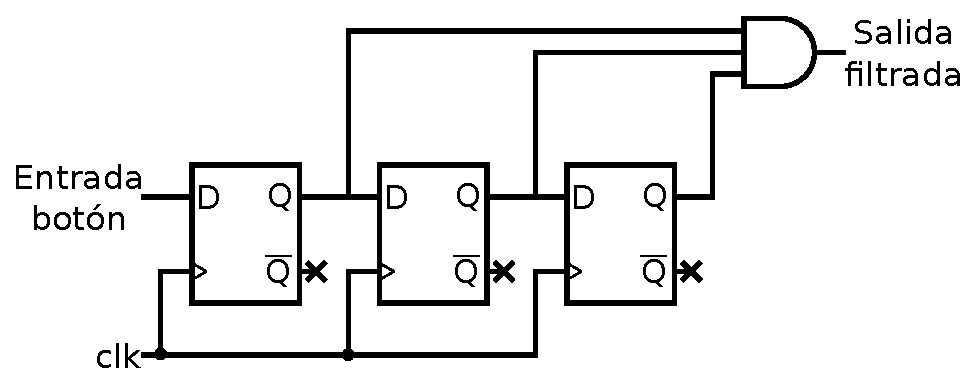
\includegraphics[width=80mm]{esquemas/debounce.eps}
    \caption{Esquema de funcionamiento del módulo btn\_debouncer}
    \label{fig:esquema-debounce}
\end{figure}

Por otro lado, como las pulsaciones del usario tienen una duración mucho mayor a la de un ciclo del reloj de control, se ha creado un segundo módulo que ante la pulsación de larga duración, envia un unico pulso con el mismo ancho que el del reloj de entrada.


%!
\subsubsection{Módulo de control maestro (main\_controller).}
Para el correcto funcionamiento del sistema, todos los módulos deben trabajar de forma coordiana, sin interferirse mutuamente. Por eso, se ha implementado este módulo, que 

Los modulos anteriormente explicados, no poseen relacion entre ellos, por tanto necesitan un módulo extra encargado de temporizar y distribuir que tareas deben realizar.

\begin{figure}[!hbt]
    \centering
    \scalebox{0.8} {\begin{tikzpicture}[auto]
    % Config
    \tikzFlow

    % Place nodes
    \node [flowStart] (idle) {Reposo};

    \node [flowDecision] at ($ (idle)+(5,-3) $) (newMsg) {Ha llegado un nuevo comando?};

    \node [flowDecision, below of=newMsg] (msgToggle) {El comando es de activación de envío de datos?};

    \node [flowDecision, below of=msgToggle] (msgSend) {El comando es de envío valor leído?};

    \node [flowDecision, below of=msgSend] (msgWrite) {El comando es de escritura de registro?};
    
    \node [flowDecision, below of=msgWrite] (msgRead) {El comando es de lectura de registro?};

    \node [flowDecision] at ($ (idle)+(0,-3) $) (newUSB) {Hay datos USB disponibles para enviar al PC?};


    \node [flowDecision] at ($ (idle)+(-5,-3) $) (push) {Se ha pulsado el botón de prueba?};
    \node [flowBase, below of=push] (testByte) {Envío de un $byte$ de prueba};





    % \node [flowStart] (idle) {Reposo};
    
    % \node [flowDecision, below of=idle] (rxLow) {Entrada del puerto serie a nivel bajo?};
    
    % \node [flowBase, below of=rxLow] (init) {Reinicio del contador de $bits$};
    
    % \node [flowBase, below of=init] (read) {Se guarda $bit$ entrante en el registro de desplazamiento};

    % \node [flowDecision, below of=read] (10bitsDone) {Se han leído los $10~bits$ del mensaje?};
    
    % \node [flowBase] at ($ (read)+(4.1,0) $) (increase) {Incremento del contador de $bits$};

    % \node [flowBase] at ($ (10bitsDone)+(4.1,0) $) (wait) {Se espera un pulso del reloj de baudios};

    % \node [flowBase, below of=10bitsDone] (save) {Se almacena el byte en memoria};

    % % % Draw edges
    % \path [flowLine] (idle) -- (rxLow);
    % \path [flowLine] (rxLow) -- (init);
    % \path [flowLine] (init) -- (read);
    % \path [flowLine] (read) -- (10bitsDone);
    % \path [flowLine] (increase) -- (read);
    
    % \node [flowHide] at ($ (idle)+(3.5,0) $) (anchor1) {};
    % \path [flowLine] (rxLow) -- node [right, xshift=-1.2cm] {Sí} (init);
    % \path [flowLine] (rxLow.east) -| node [above, xshift=-1.2cm] {No} (anchor1.center);
    
    % \path [flowLine] (save.east) -| +(4.5,0) |- (idle.east);
    
    % \path [flowLine] (wait) -- (increase);
    % \path [flowLine] (10bitsDone.east) node [above, xshift=0.2cm] {No} -- (wait);
    % \path [flowLine] (10bitsDone) -- node [right, xshift=-1.2cm] {Sí} (save);
\end{tikzpicture}}
    \caption{Diagrama de funcionamiento del módulo de control maestro}
    \label{fig:flujo_main_controller}
\end{figure}

%!
\subsection{Simulaciones finales.}
Con el objetivo de eliminar posibles errores capaces de dañar los propios componentes \emph{hardware}, y para comprobar el correcto funcionamiento del sistema, se han realizado diversas pruebas previas al sintetizado y utilización de la configuración final.

\begin{enumerate}
    %! Revisar
    \item \textbf{Pruebas de botones auxiliares.}
    Se simulan las pulsaciones de los botones externos de la \emph{FPGA}, produciendo un reinicio con el primero, y un envío de un $byte$ por el puerto serie con el segundo.

    %! Revisar
    \item \textbf{Prueba de lectura de registro.}
    Se simula una petición enviada por el puerto serie, que realice una lectura de registro \emph{ULPI}.
    
    %! Revisar
    \item \textbf{Prueba de transmisión del último registro leído.}
    Se simula una petición enviada por el puerto serie para enviar el valor del registro anteriormente leído al PC.
    
    %! Revisar
    \item \textbf{Prueba de escritura de registro.}
    Se simula una petición enviada por el puerto serie, que escriba un $byte$ en un registro del integrado \emph{USB3300}.
    
    %! Revisar
    \item \textbf{Prueba de captación de 6 bytes USB.}{\label{enum:captacion_6}}
    Prueba en la que se simula la llegada de $6~bytes$ de datos USB, se comprueba también el correcto guardado de los mismos en la memoria interna de la \emph{FPGA}.
    
    %! Revisar
    \item \textbf{Prueba de activación de la transmisión de datos capturados.}{\label{enum:activacion_transmision}}
    Se simula una petición enviada por el puerto serie, con la que activar el envío automático de los datos capturados.
    
    %! Revisar
    \item \textbf{Prueba de captación de 4 bytes USB.}
    De igual manera que la prueba \ref{enum:captacion_6}, pero enviando esta vez $4~bytes$ con el envio de datos al PC activado.
    
    %! Revisar
    \item \textbf{Prueba de captación de cambios de estado del bus USB.}
    Se simula un cambio de estado USB enviado por el bus \emph{ULPI}, observando si se actualiza en la \emph{FPGA}.
    
    %! Revisar
    \item \textbf{Prueba de finalización de la transmisión de datos capturados.}
    De igual manera que en la prueba \ref{enum:activacion_transmision} se activaba el envió de datos automático, se realiza la misma petición, desactivandolo en este caso.
\end{enumerate}


%!
\subsection{Información del sintetizado final.}




%!
\section{Resultados del \emph{software} de control y guardado.}
\noWord[Comentar más de esta frase, ya que la utilizo mas adelante] El sistema en su conjunto no sería funcional, sin una aplicación que utilice los recursos creados para recibir y almacenar la captura.



%! Revisar
\subsection{Aplicaciones de utilidad.}
% lenguaje, hilos, librerías, etc...
A medida que se ha ido desarrollando la parte \emph{hardware}, se han creado varias utilidades en lenguaje \emph{Python}, con las que realizar cálculos de forma rápida o con las que comprobar el funcionamiento de ciertas partes del sistema. Hay que destacar:
\begin{enumerate}
    %* Comprobar
    \item \textbf{Utilidad de divisiones del reloj.} \\
    Utilidad con la que poder realizar de forma rápida varios cálculos relacionados con los relojes de entrada. Por ejemplo, obtener los valores óptimos con los que dividir un reloj para generar unos baudios deseados. En el listado \ref{src:utilidad_divisiones_reloj_out}, se plasma un ejemplo de uso.
    \begin{lstlisting}[
        caption={Ejemplo de la utilidad de divisiones de reloj.},
        label=src:utilidad_divisiones_reloj_out]
$ ./get_divider.py
  Usage: ./get_divider.py [option] arg1 arg2
  Options: 
      -o: Print the optimal counter value for a given clock (arg1) and Serial baudrate (arg2). [Default]
      -b: Print the minimal divider value for a given clock (arg1) and Serial baudrate (arg2).
      -d: Print the minimal divider value for a given clock (arg1) and time (arg2).
      -t: Print the time (and serial baudrate) for a given clock (arg1) and divider (arg2).
      -a: Print, for a given clock (arg1), all the possible periods that can be generated between 0 and arg2.
      -c: Print the clock for a given time (arg1) and divider (arg2).
$ ./get_divider.py -o 12000000 115200
  Optimal counter value: 105
$ ./get_divider.py -b 12000000 9600
  Recomended divider (with 18% error): 10 [8.533333333333334e-05s]
  10 [8.533333333333334e-05s] - [0.00010416666666666667s] - 11 [0.00017066666666666668s]          
    \end{lstlisting}
    
    %! Revisar
    \item \textbf{Utilidad de generación de baudios.} \\
    Pequeña aplicación que, para los $baudios$ más comunes, genere varias definiciones de \emph{Verilog} a usar por el módulo encargado de generar el reloj de baudios. En el listado \ref{src:utilidad_baudios_out} se muestra un ejemplo de la salida de la aplicación.
%     \\ \noWord[Borrar listado??? La verdad, es algo inutil ponerlo]
%     \begin{lstlisting}[
%         caption={Ejemplo de la utilidad de generación de baudios ante \emph{60 MHz} de entrada.},
%         label=src:utilidad_baudios_out]
% $ ./gen_bauds.py
%   `define B921600 66
%   `define B460800 131
%   `define B256000 235
%   `define B230400 261
%   `define B153600 391
%   `define B128000 469
%   `define B115200 521
%   `define B57600  1042
%   `define B56000  1072
%   `define B38400  1563
%   `define B28800  2084
%   `define B19200  3125
%   `define B14400  4167
%   `define B9600   6250
%   `define B4800   12500
%   `define B2400   25000
%   `define B1200   50000
%   `define B600    100000
%   `define B300    200000
%   `define B110    545455
%     \end{lstlisting}
    
    %! Revisar
    \item \textbf{Utilidad de control serie.} \\
    Aplicación, que usando la librería encargada de controlar puertos serie, compruebe el funcionamiento del protocolo. Se puede configurar para abrir el puerto serie a cualquier velocidad, y poder enviar comandos de prueba.
\end{enumerate}

%!
\subsection{Información de la aplicación.}
Tal como se ha comentado al principio de esta sección, aun teniendo mayor carga la parte \emph{hardware}, es esencial implementar una aplicación que se comunique con la FPGA y permita su funcionamiento.

Para ello, utilizando lenguaje C, se ha creado una aplicación que dando opciones de control con una simple interfaz, es capaz de enviar comandos o recibir datos USB, y a su vez, es capaz de almacenarlos para su posterior uso o estudio.

La aplicación se ha dividido de la siguiente manera:
\begin{enumerate}
    %!
    \item \textbf{Hilo encargado de controlar las entradas de usuario.} \\
    Tanto la configuración a usar para conectarse a la \emph{FPGA} (puerto serie y baudios), como los comandos a enviar, son introducidos al programa por medio de un simple menú.

    \begin{lstlisting}[
        caption={Ejemplo de la utilidad de generación de baudios ante \emph{60 MHz} de entrada.},
        label=src:utilidad_]
$ .sddf
    \end{lstlisting}
    
    %!
    \item \textbf{Hilo encargado de gestionar la comunicación con la \emph{FPGA}, así como almacenar la trama capturada.}
    Por un lado, este hilo envio los comandos introducidos por el usuario a la FPGA, y por otro, cuando llegen los datos USB capturados, estos son almacenados en un archivo.
\end{enumerate}


%!
\subsection{Información del archivo generado.}
% Info JSON, como interpretarlo, imagen de ejemplo, etc...
Se ha elegido almacenar la información captruada en un archivo formato JSON\footnote{INFO JSON}, 

\begin{lstlisting}[
    caption={Ejemplo de la utilidad de generación de baudios ante \emph{60 MHz} de entrada.},
    label=src:utilidad_]
$ .sddf
\end{lstlisting}


%!
\subsection{Conversión de JSON a PCAP.}
% Info JSON, como interpretarlo, imagen de ejemplo, etc...
Para poder analizar la captura en la aplicación \emph{Wireshark}, se ha creado otra utilidad, que a partir del archivo JSON generado anteriormente, lo transforma a PCAP.






% \chapter{Resultados}
% \label{ch:resultados-plantilla}

% Escribe en este capítulo los resultados del proyecto.  Este capítulo debería explicar los resultados de forma global, no los resultados de cada iteración.  Probablemente será el capítulo con más tablas y gráficas.  Revisa las secciones~\ref{sec:figuras} y~\ref{sec:tablas} para aprender cómo se escriben en \LaTeX{}.